\documentclass{standalone}
\usepackage{forsyde-tikz}
\usepackage{forsyde-plot}

\begin{document}

\newsavebox\insig
\sbox{\insig}{
  \begin{de-signal}[%
    timestamps=2, tag scale=.6]{9}
    \tiny
    \nextsignal{}  \present{2}{1} \present{3}{2} 
        \present{1}{3} \present{2}{4} \present{1}{5} \infinity
  \end{de-signal}
}
\newsavebox\outsig
\sbox{\outsig}{
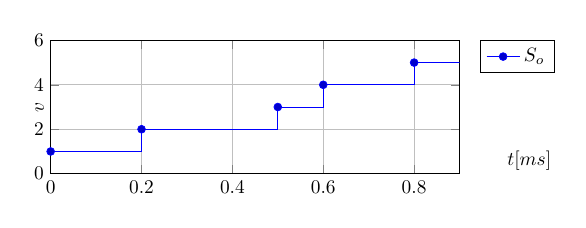
\begin{tikzpicture}[scale=.7]
  \begin{axis}[
    height=4cm, width=9cm,
    xlabel={$t[ms]$}, ylabel=$v$,
    xmin=0, xmax=0.9, ymin=0, ymax=6, 
    grid=major,
    x label style={
      at={(axis description cs:1.1,.1)},anchor=west},
    y label style={
      at={(axis description cs:0,.5)}},
    legend style={at={(1.05,1)}, anchor=north west},
    ]
    \addplot+[const plot] coordinates {
      (0,1) (0.2,2) (0.5,3) (0.6,4) (0.8,5) (2,5)}; 
    \addlegendentry{$S_o$}
  \end{axis} 
\end{tikzpicture}
}


\begin{tikzpicture}[nomoclabel]
  \leafstd[moc=de, ni=1, no=1, nf=1, f1={$0.1$ms}, type=toCT]{c1} {0,0} {}; 
  \node[anchor=east] (i1) at ($(c1-p.i1)-(1,0)$) {\usebox{\insig}}; 
  \node[anchor=west] (o1) at ($(c1-p.o1)+(2,0)$) {\usebox{\outsig}};
  \node[anchor=west] (o1l) at ($(c1-p.o1)+(1,0)$) {$S_o$};

  \signal[] (i1) -> (c1-p.i1); 
  \signal[] (c1-p.o1) -> (o1l);
  % \signal[-|-=.2] (c1-p.o2) -> (o2.north east);
\end{tikzpicture}  
\end{document}

%%% Local Variables:
%%% mode: latex
%%% TeX-master: t
%%% End:
